\clearpage
% \ifx \notincludehead\undefined
\normalsize
\end{document}
\fi


\newpage
\subsection{Управление и диспетчеризация производства}
\label{bp:production}

% На производстве работает 16 машинистов, 2 погрузчика (водителя), 1 грузчик, 1 инженер технолог, 1 инженер качества, 1 комплектовщик оснастки, 1 мастер смены.


Производство работает в одну смену. 





\textbf{Выработка гофроагрегата}


Мастер смены выдает задание на ГА (рис. \ref{pic:f29}). Машинист вбивает данные на продольной и поперечной резках в систему управления заказами на гофроагрегате Hsieh Hsu.

Бригадир передает в устной форме на склад запрос на поставку необходимого сырья, предварительно посмотрев <<домоты>> (остатки по рулонам). Бригадир совместно с кладовщиком заполняют ведомость по сырью (рис. \ref{pic:f26}). Переданный на производство со склада рулон сразу списывается с учета.


Машинисты запускают ГА, производят гофрокартон согласно  планового задания. 

Данные по выработке вносят в MS EXCEL (рис. \ref{pic:f23}).

Бирки на полуфабрикаты, выпущенные на ГА, машинисты печатают (рис. \ref{pic:f31}) сразу на весь заказ. Бирки печатаются непосредственно на ГА. Механизм автоматического формирования бирок не настроен.

По факту выработки с гофроагрегата машинист формирует отчет по выработке по форме (рис. \ref{pic:d6}).




\textbf{Выработка линии переработки}

Мастер смены выдает машинистам задания по линиям (рис. \ref{pic:f24}). Технологические карты бригадиры печатают с сервера. 
Краску, при возникновении необходимости, выдает колорист.
Оснастку машинисты берут сами. Оснастка хранится около производственных линий.
Машинисты настраивают машину и выпускают продукцию согласно требованиям ТК.


Бирки на готовую продукцию печатает мастер сразу на весь заказ и с плановым заданием передает на линию (рис. \ref{pic:f30}).

Выработку машинисты на линиях вносят в файл MS EXCEL  (рис. \ref{pic:f23}).


Бригадиры на перерабатывающих линиях ведут таблицу MS EXCEL с указанием простоев (рис. \ref{pic:f28}. Подробнее процесс описан в разделе \ref{bp:maintance}).

В конце смены на основании данных по выработкам из таблицы MS EXCEL мастер заполняет отчет производства за смену (рис. \ref{pic:f25}).

Также мастер заполняет ведомость передачи ГП на склад и сверяется с данными кладовщика готовой продукции (рис. \ref{pic:f6}).




\begin{figure}
\begin{center}
 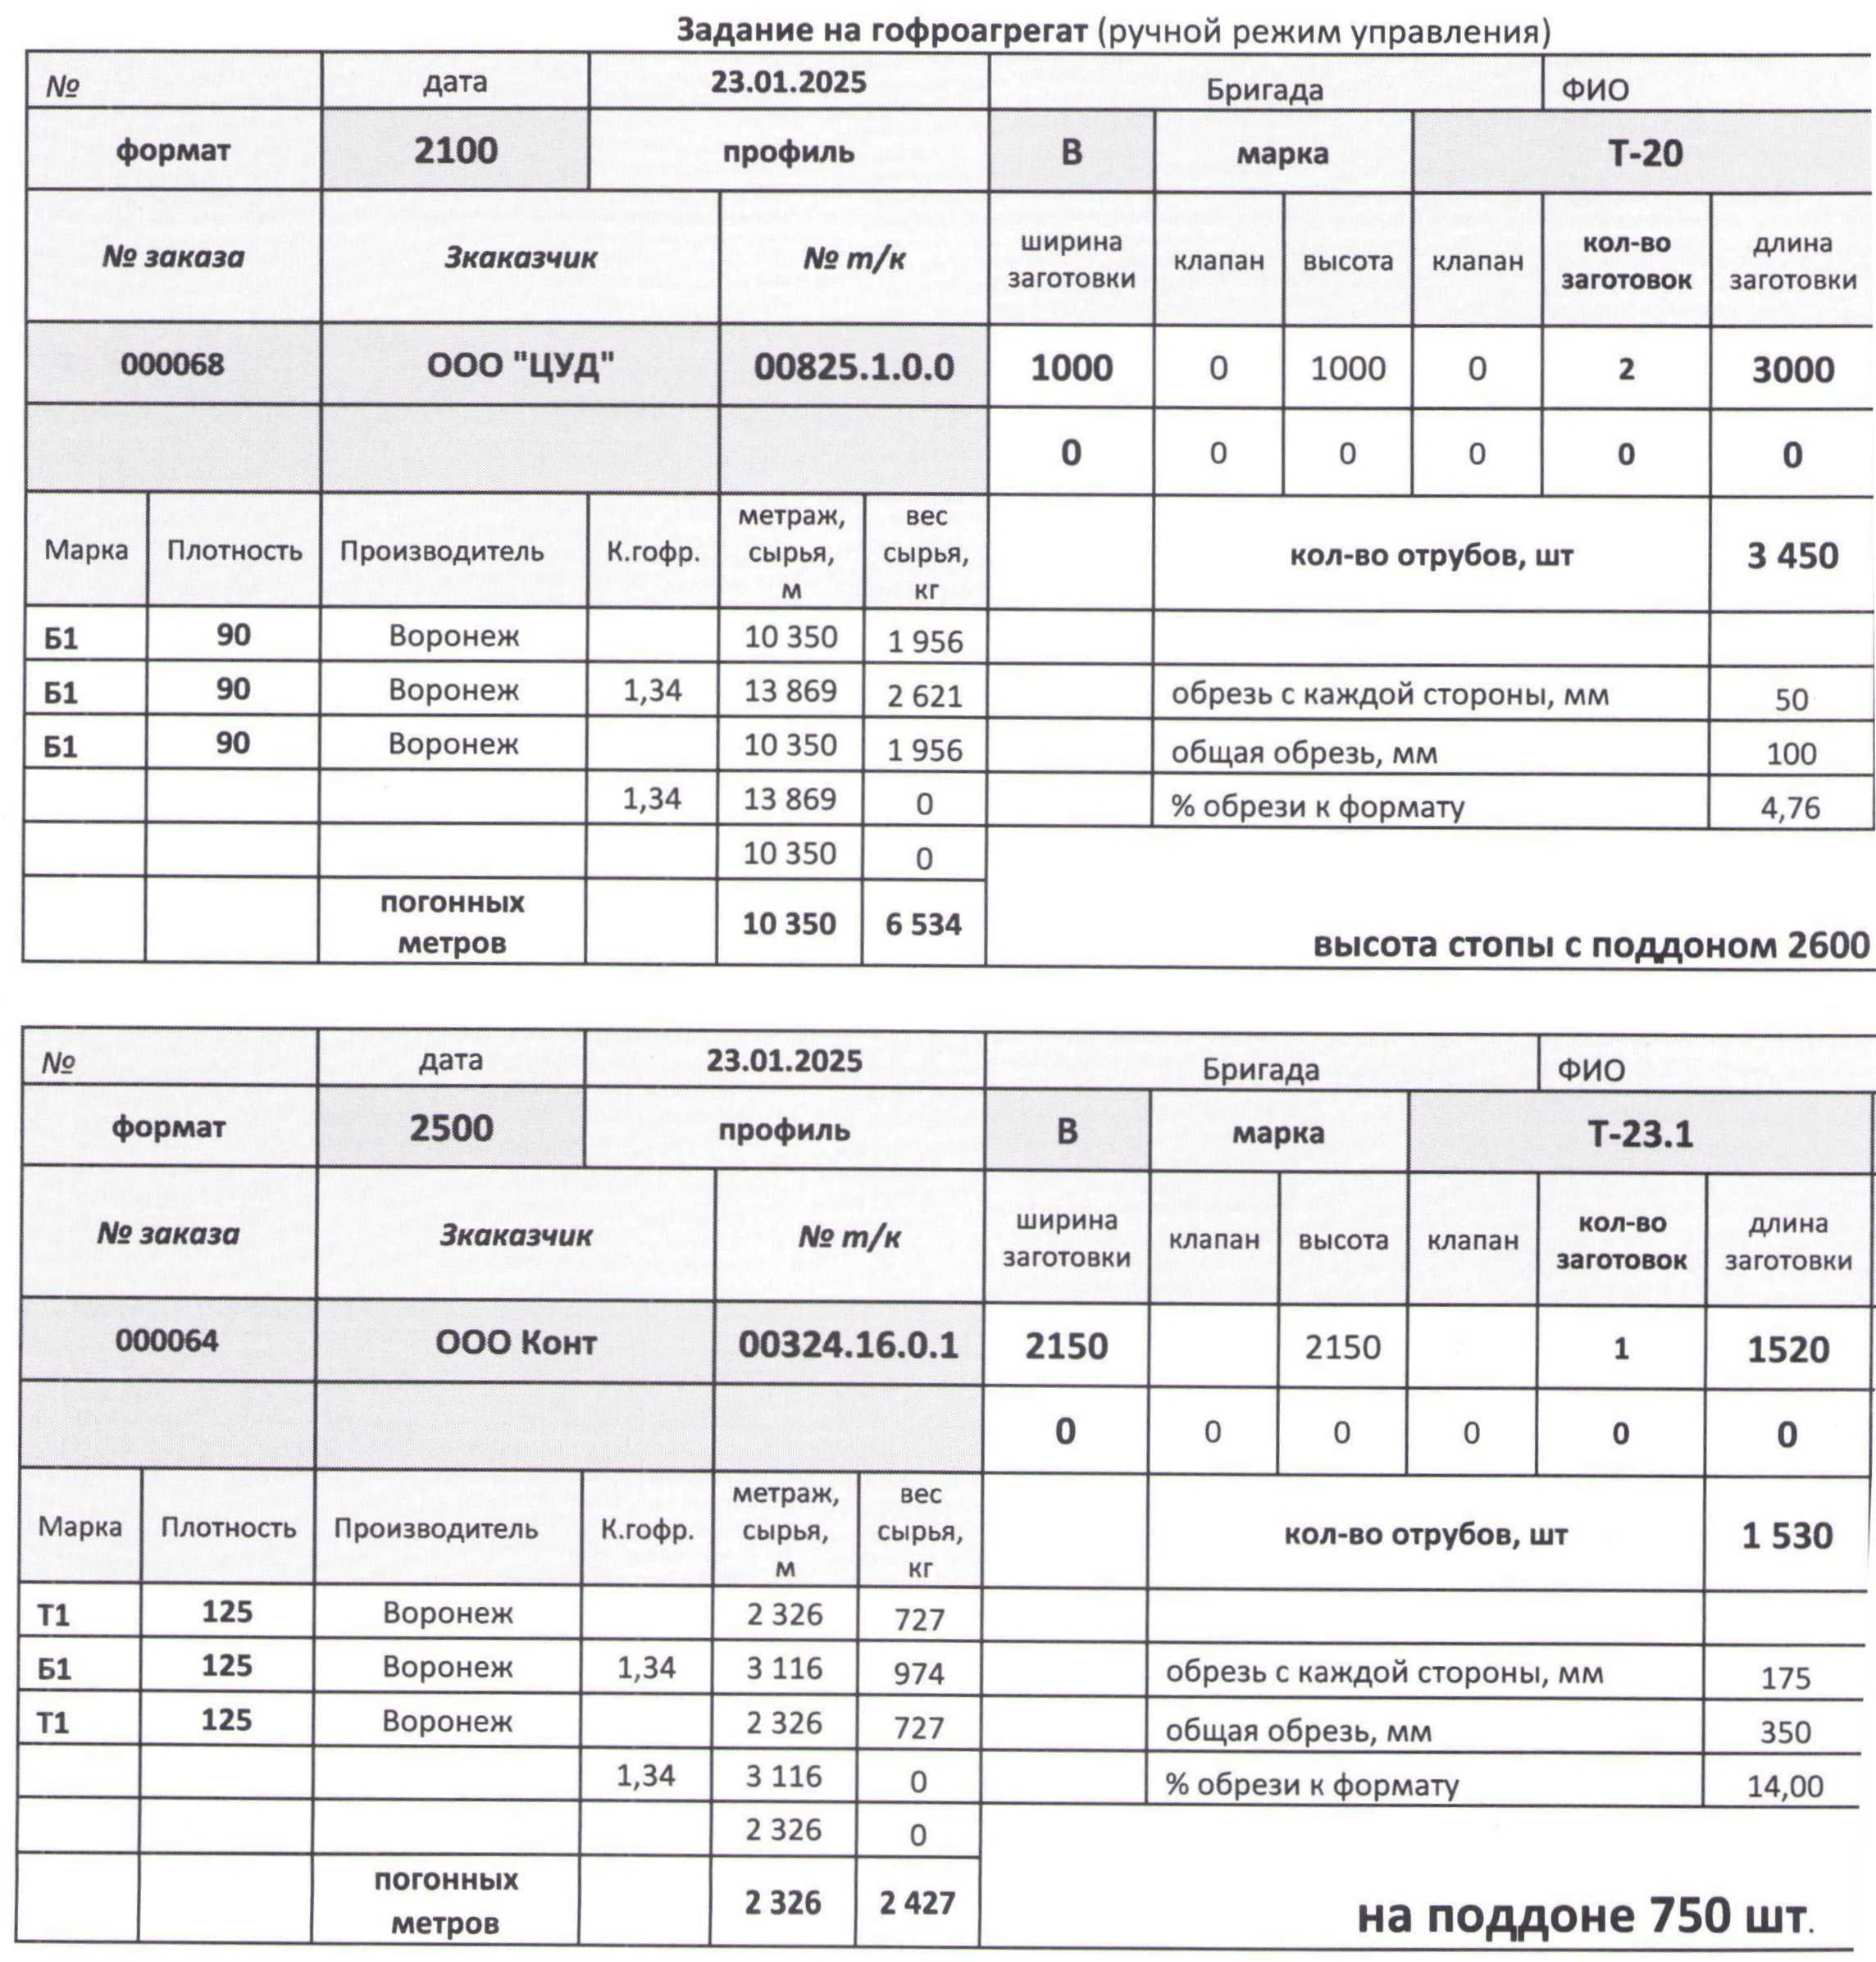
\includegraphics[width=\linewidth, height=0.94\textheight, keepaspectratio]{Pics/f29.jpg}
\end{center}
\caption{Задание на смену для ГА}
\label{pic:f29}
\end{figure}

\begin{figure}
\begin{center}
 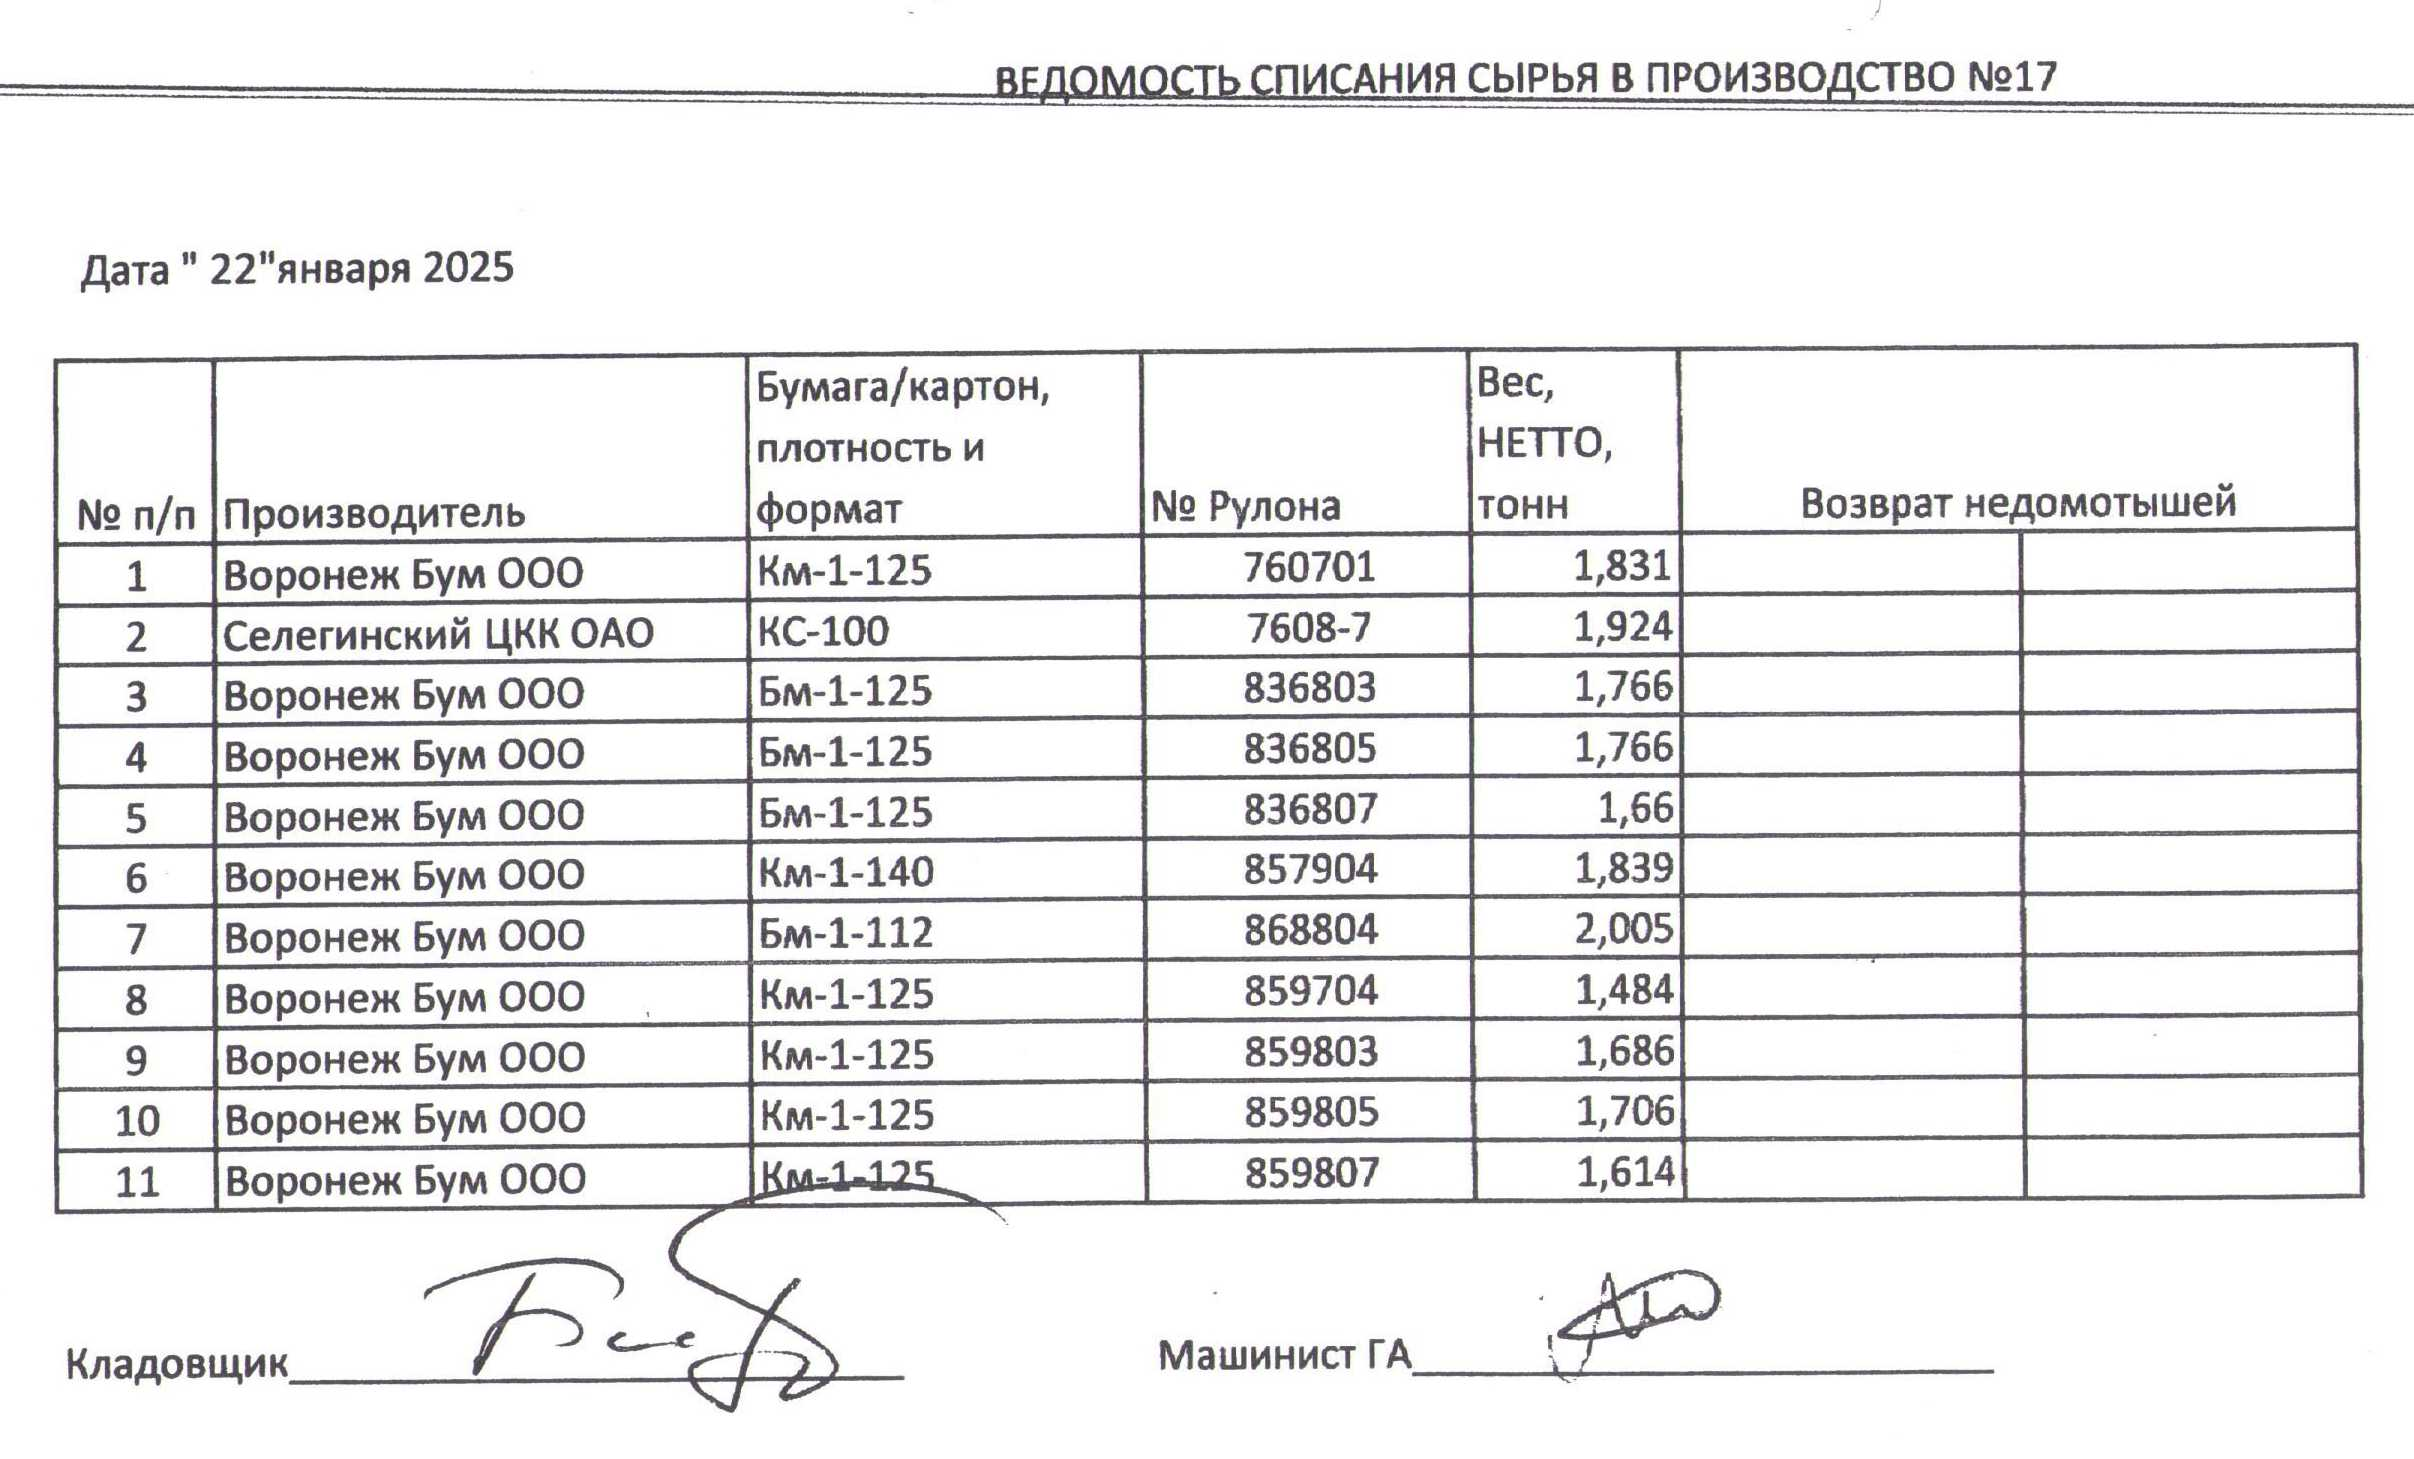
\includegraphics[width=\linewidth, height=0.94\textheight, keepaspectratio]{Pics/f26.jpg}
\end{center}
\caption{Ведомость по сырью}
\label{pic:f26}
\end{figure}

\begin{figure}
\begin{center}
 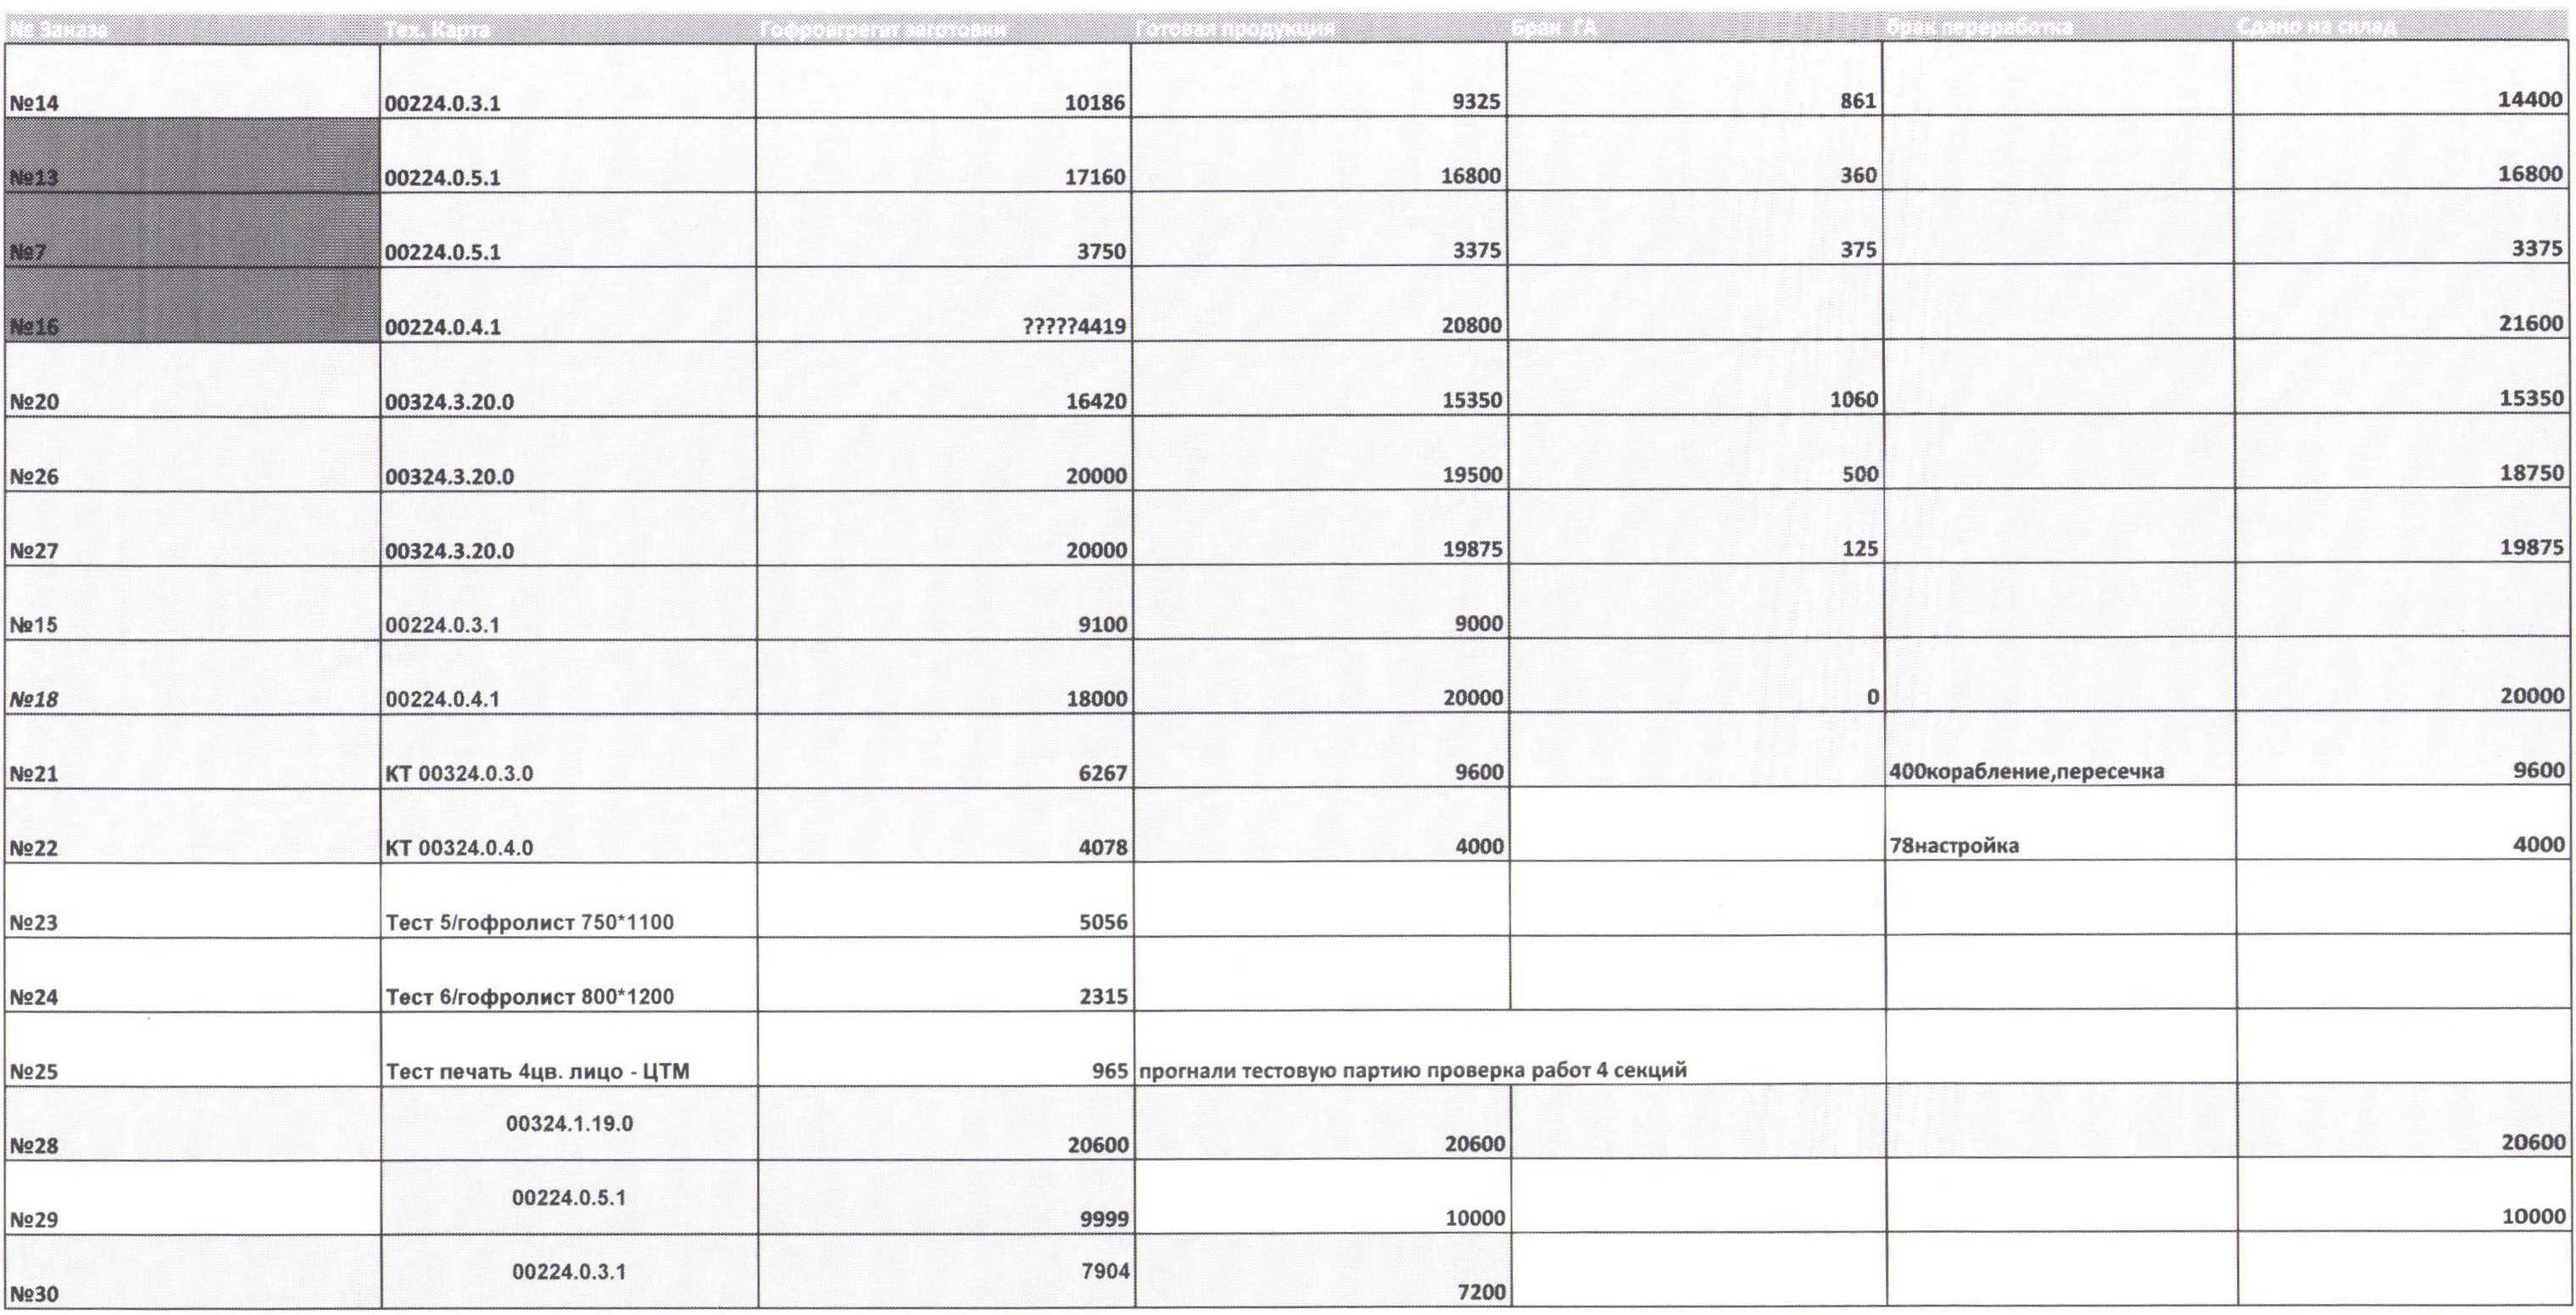
\includegraphics[width=\linewidth, height=0.94\textheight, keepaspectratio]{Pics/f23.jpg}
\end{center}
\caption{Учет выработки}
\label{pic:f23}
\end{figure}

\begin{figure}
\begin{center}
 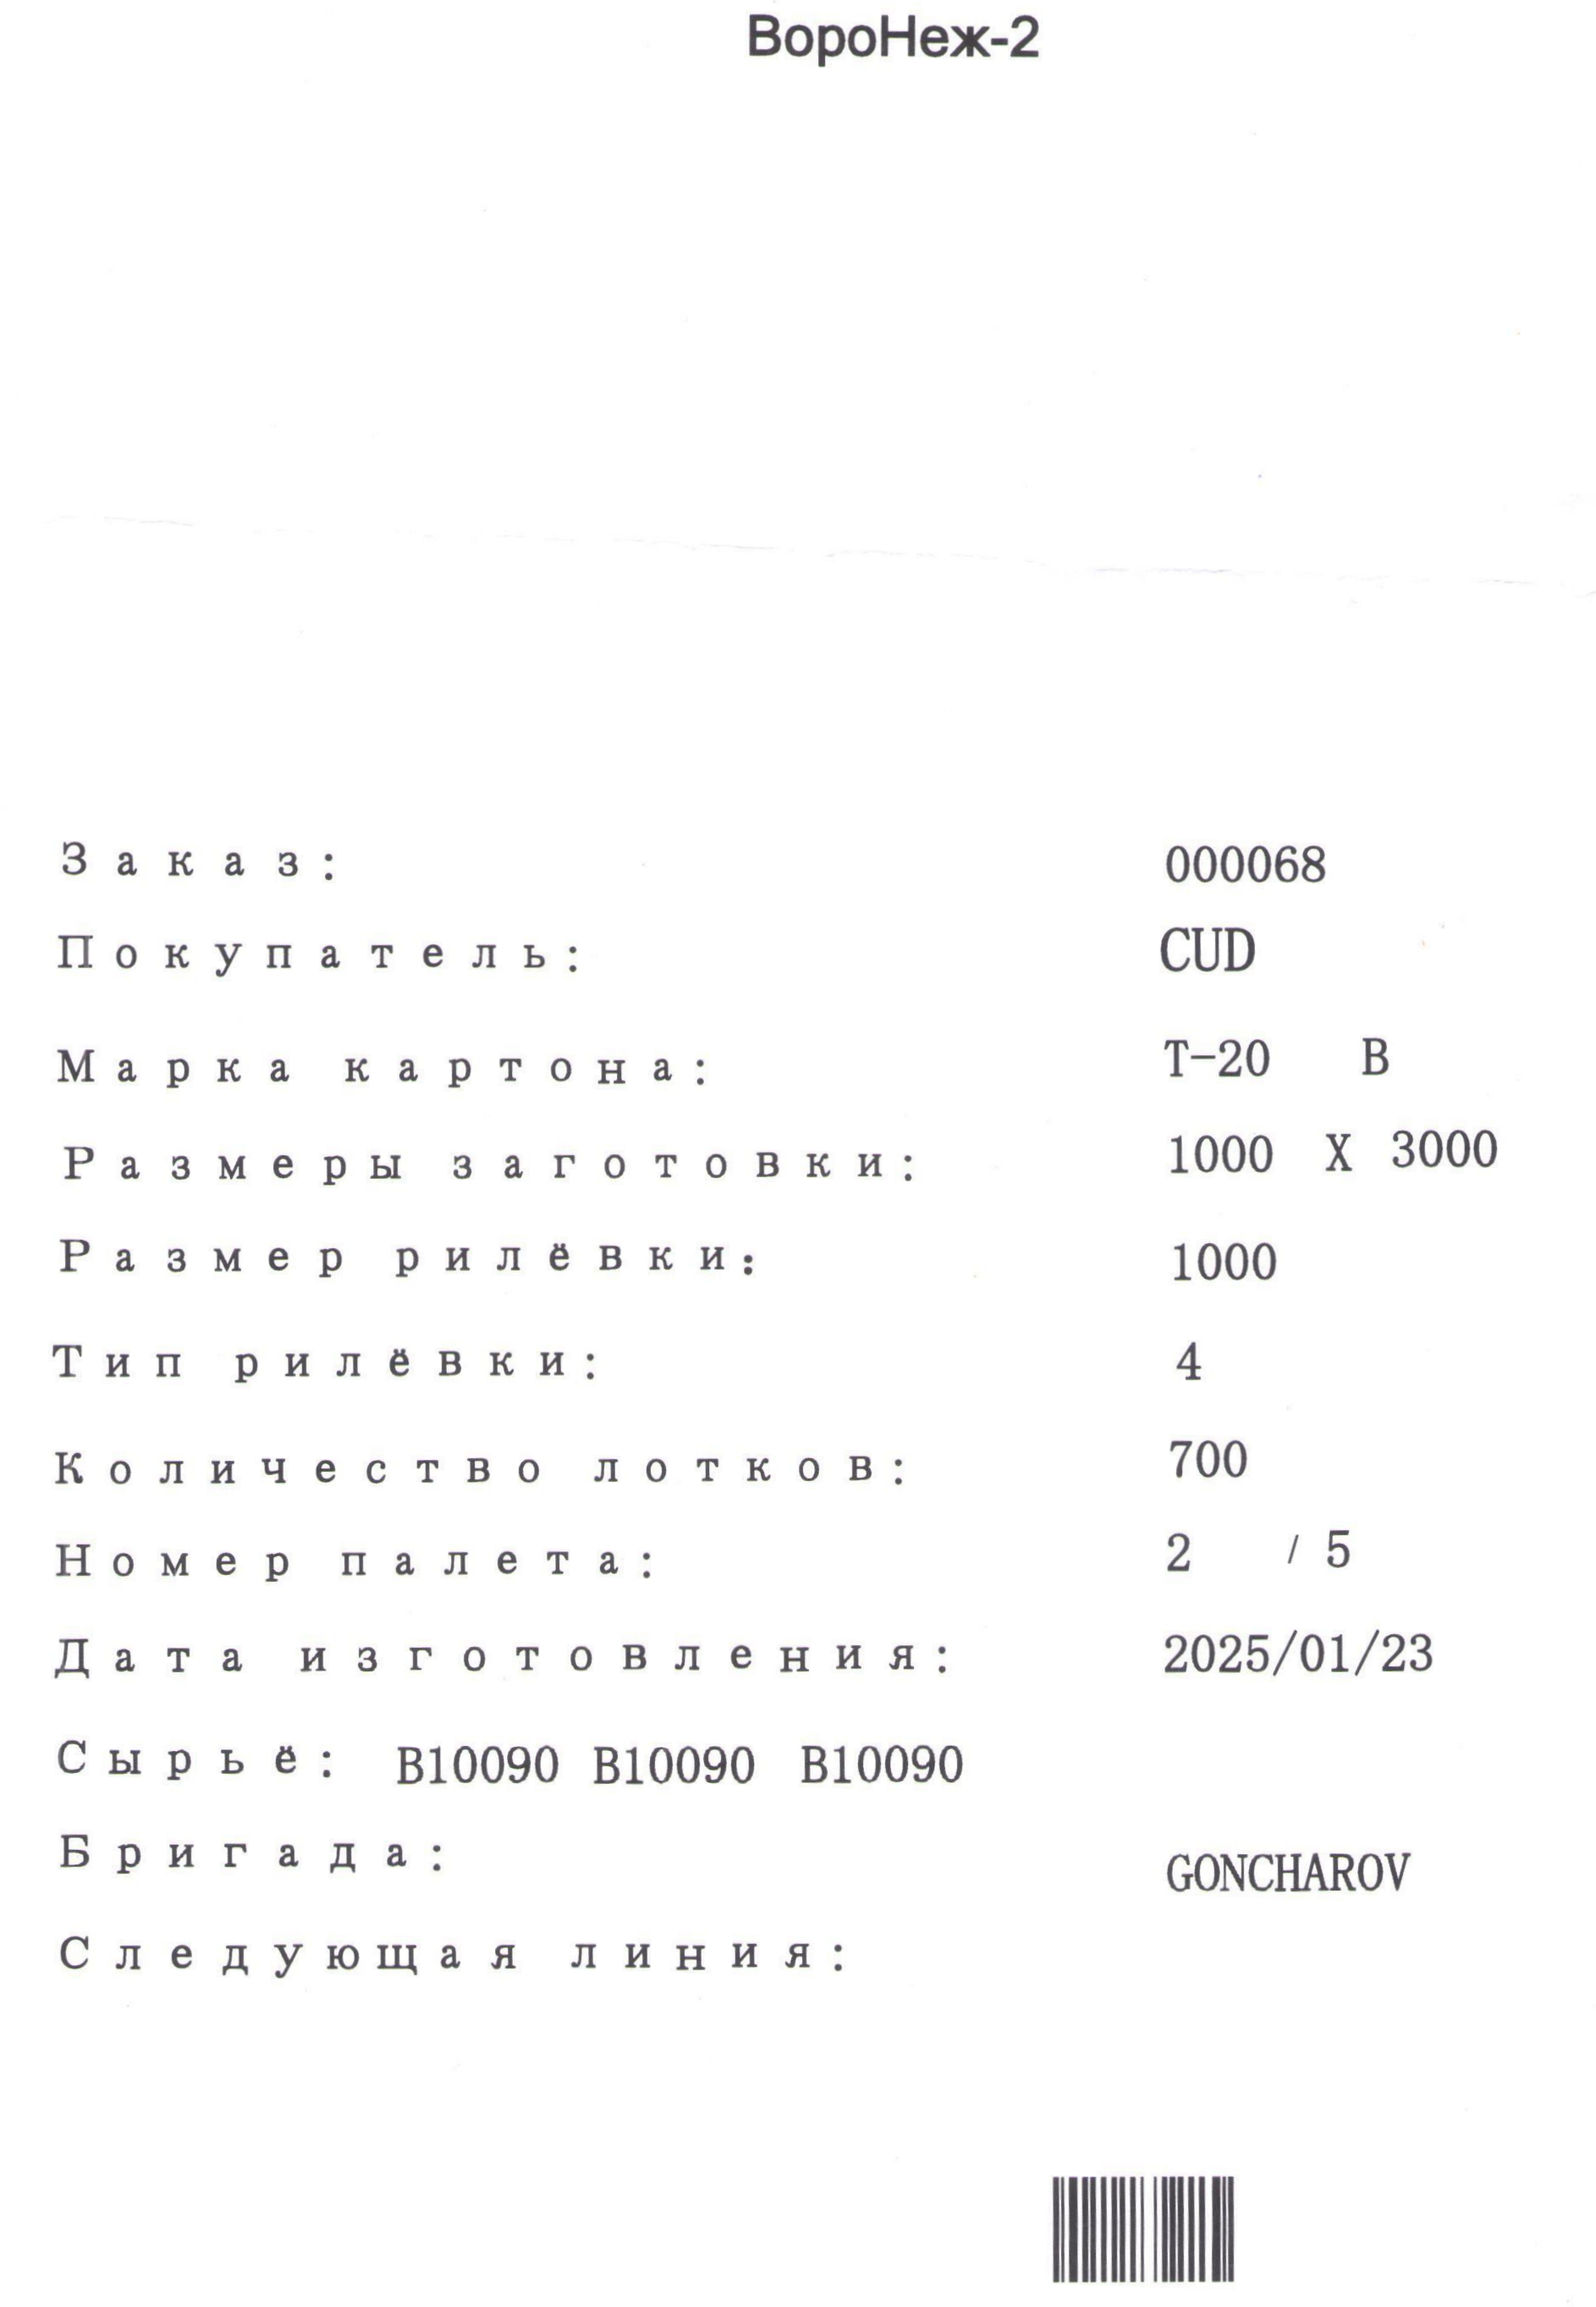
\includegraphics[width=\linewidth, height=0.94\textheight, keepaspectratio]{Pics/f31.jpg}
\end{center}
\caption{Бирки на ПФ}
\label{pic:f31}
\end{figure}

\begin{figure}
\begin{center}
 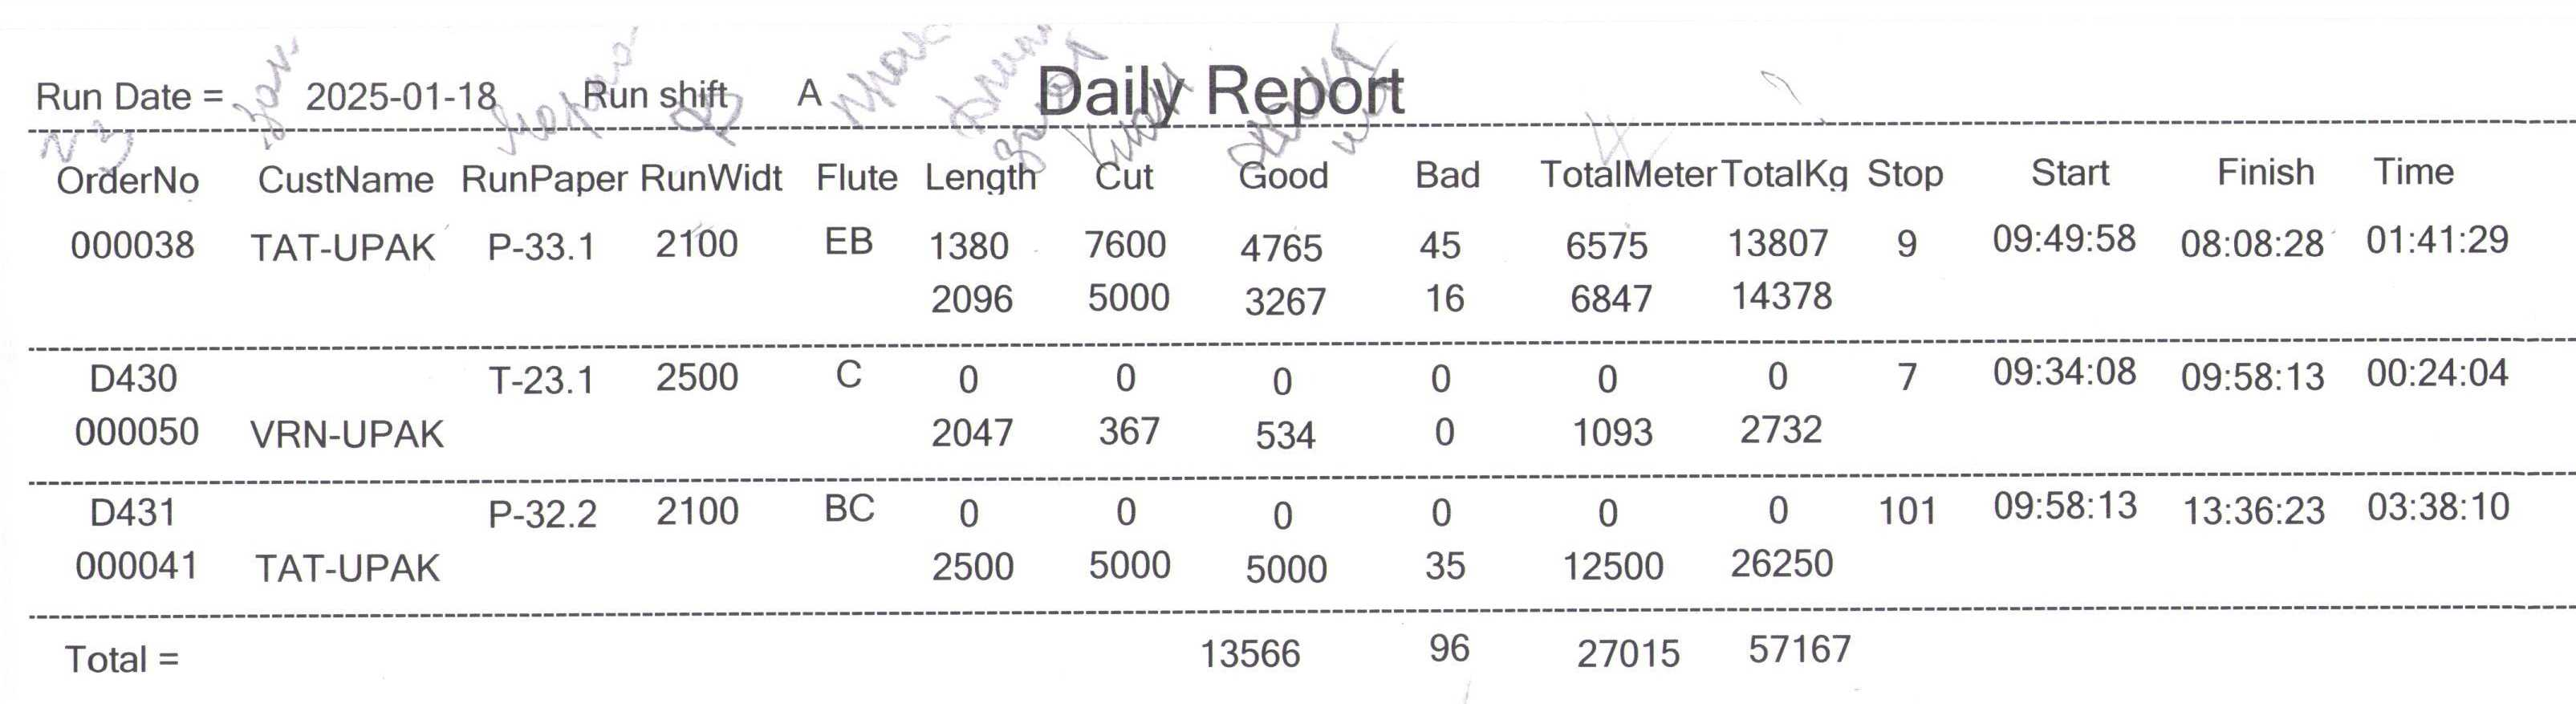
\includegraphics[width=\linewidth, height=0.94\textheight, keepaspectratio]{Pics/d6.jpg}
\end{center}
\caption{Отчет производства за смену ГА}
\label{pic:d6}
\end{figure}

\begin{figure}
\begin{center}
 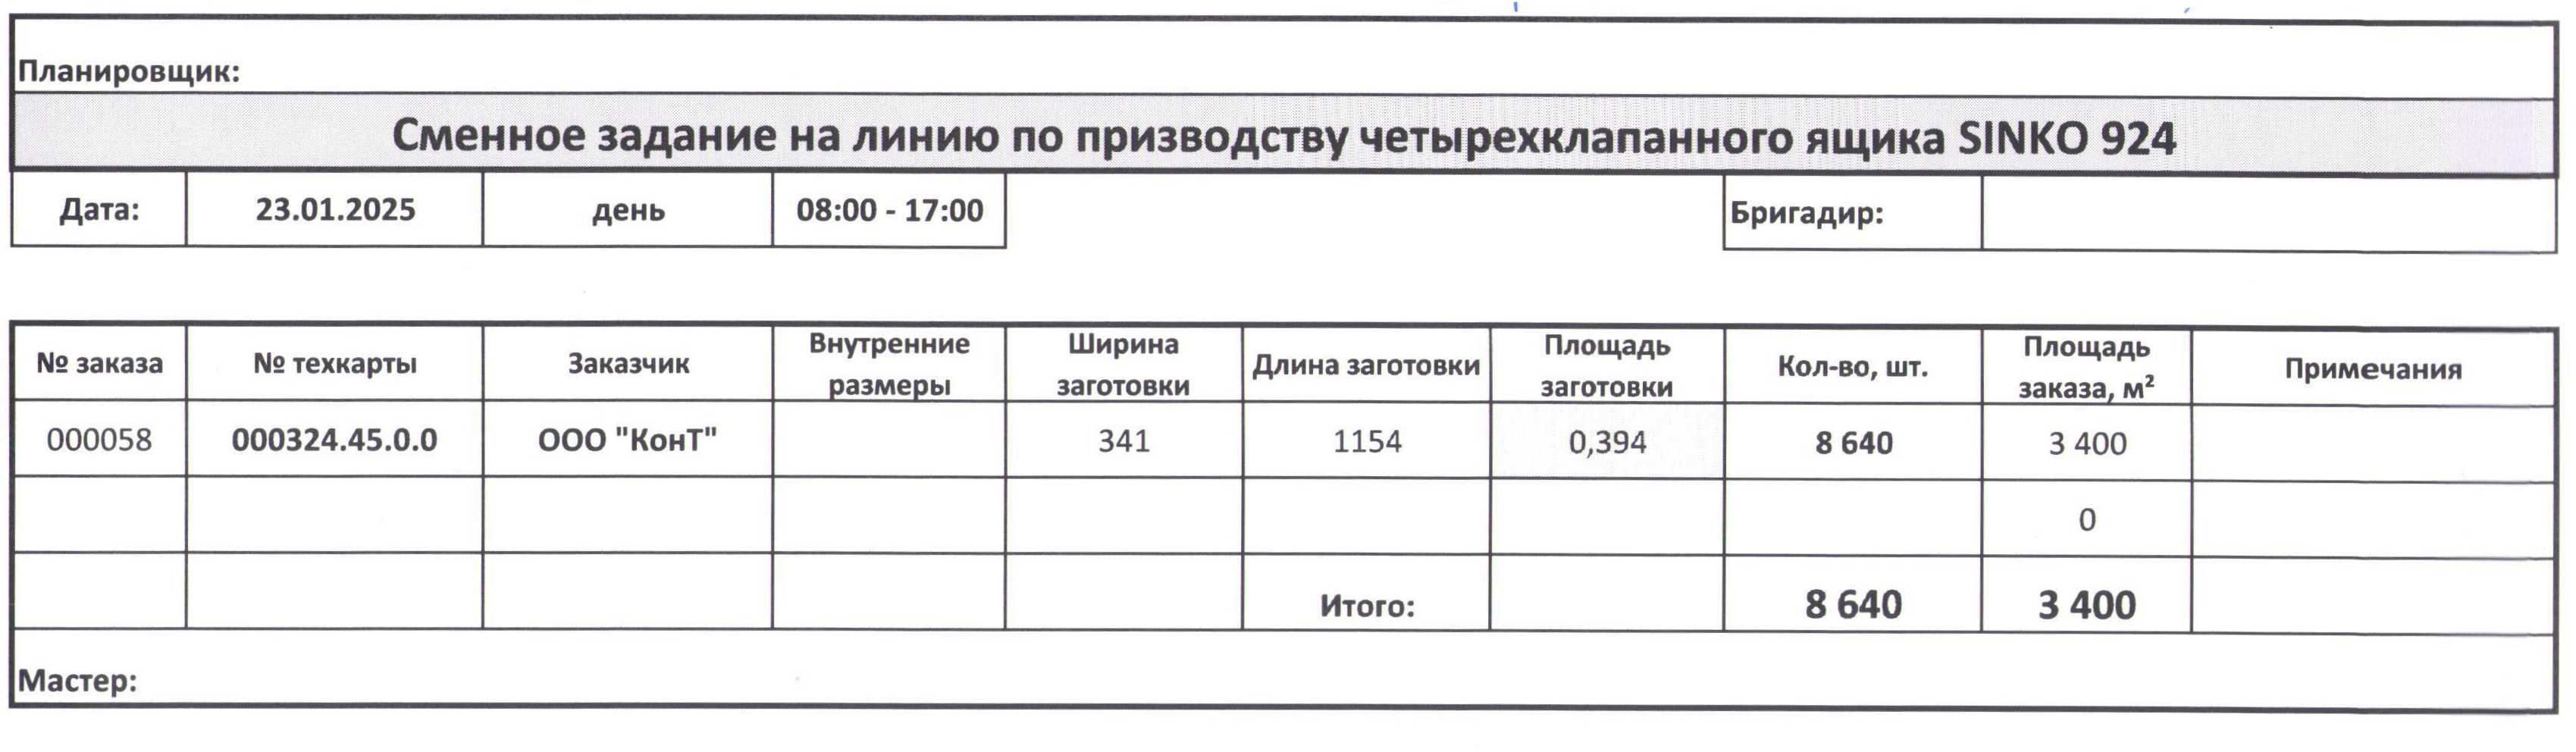
\includegraphics[width=\linewidth, height=0.94\textheight, keepaspectratio]{Pics/f24.jpg}
\end{center}
\caption{Задание на смену для ПЛ}
\label{pic:f24}
\end{figure}

\begin{figure}
\begin{center}
 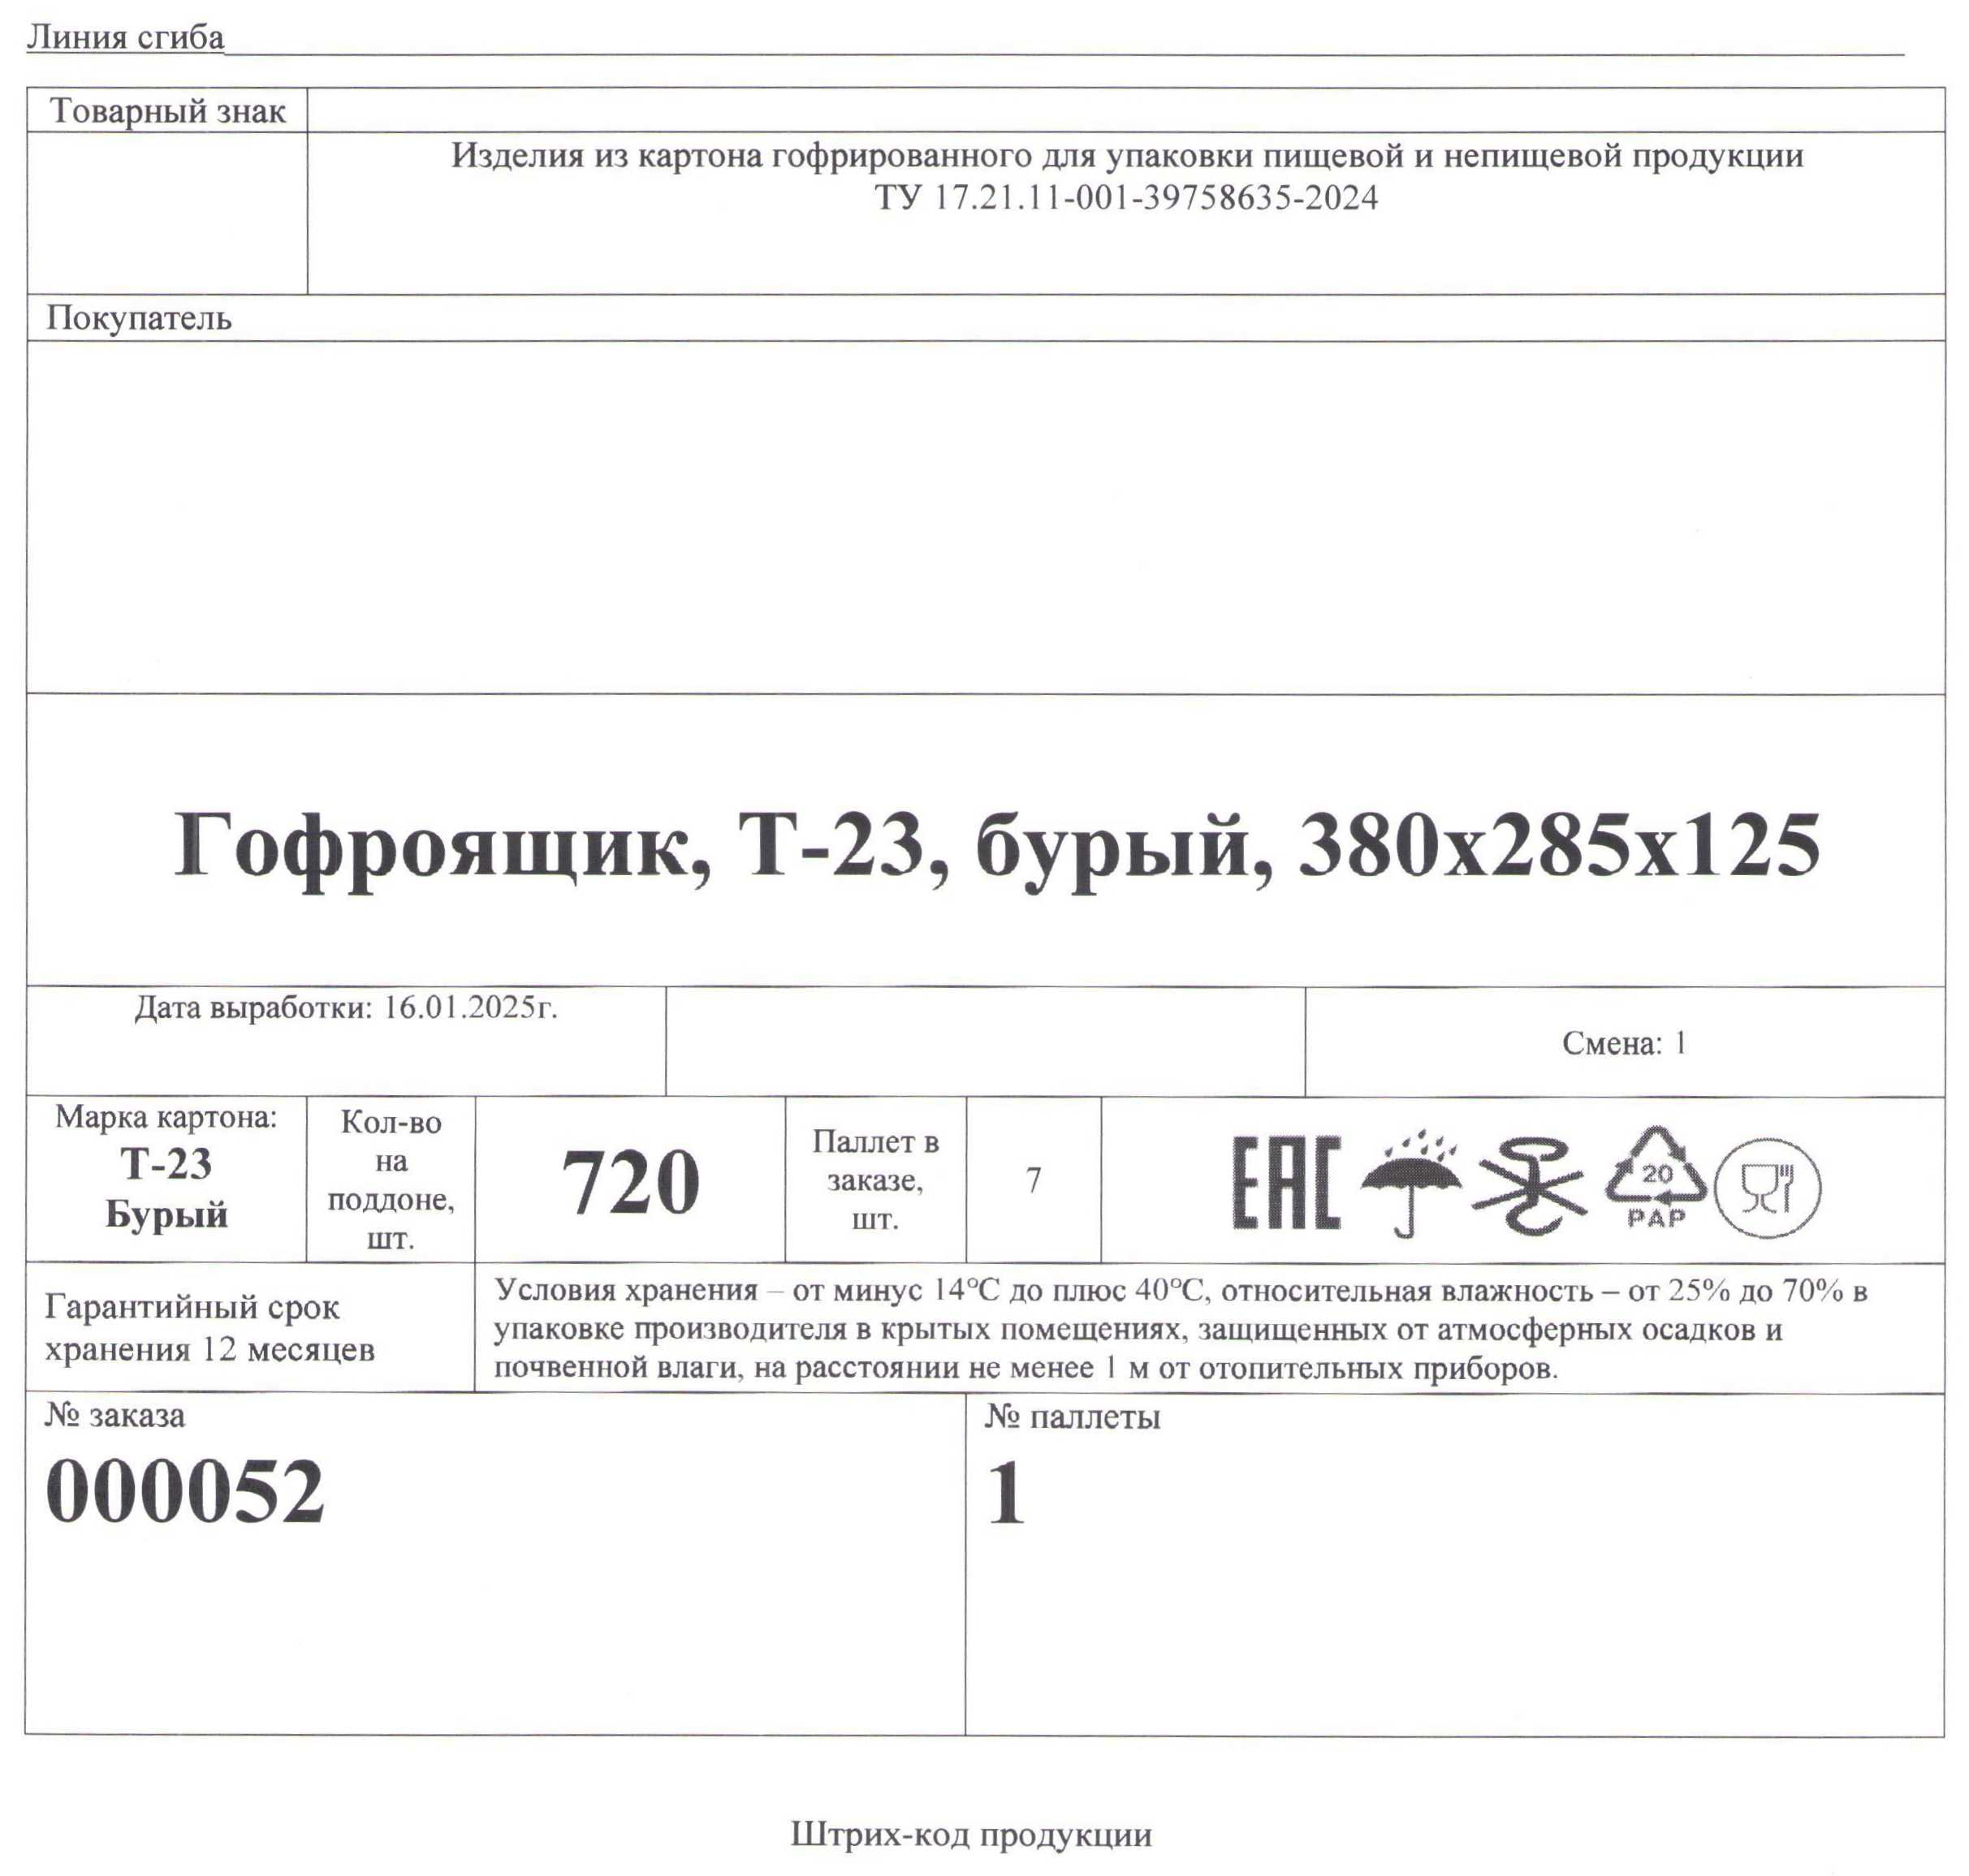
\includegraphics[width=\linewidth, height=0.94\textheight, keepaspectratio]{Pics/f30.jpg}
\end{center}
\caption{Бирки на ГП}
\label{pic:f30}
\end{figure}

\begin{figure}
\begin{center}
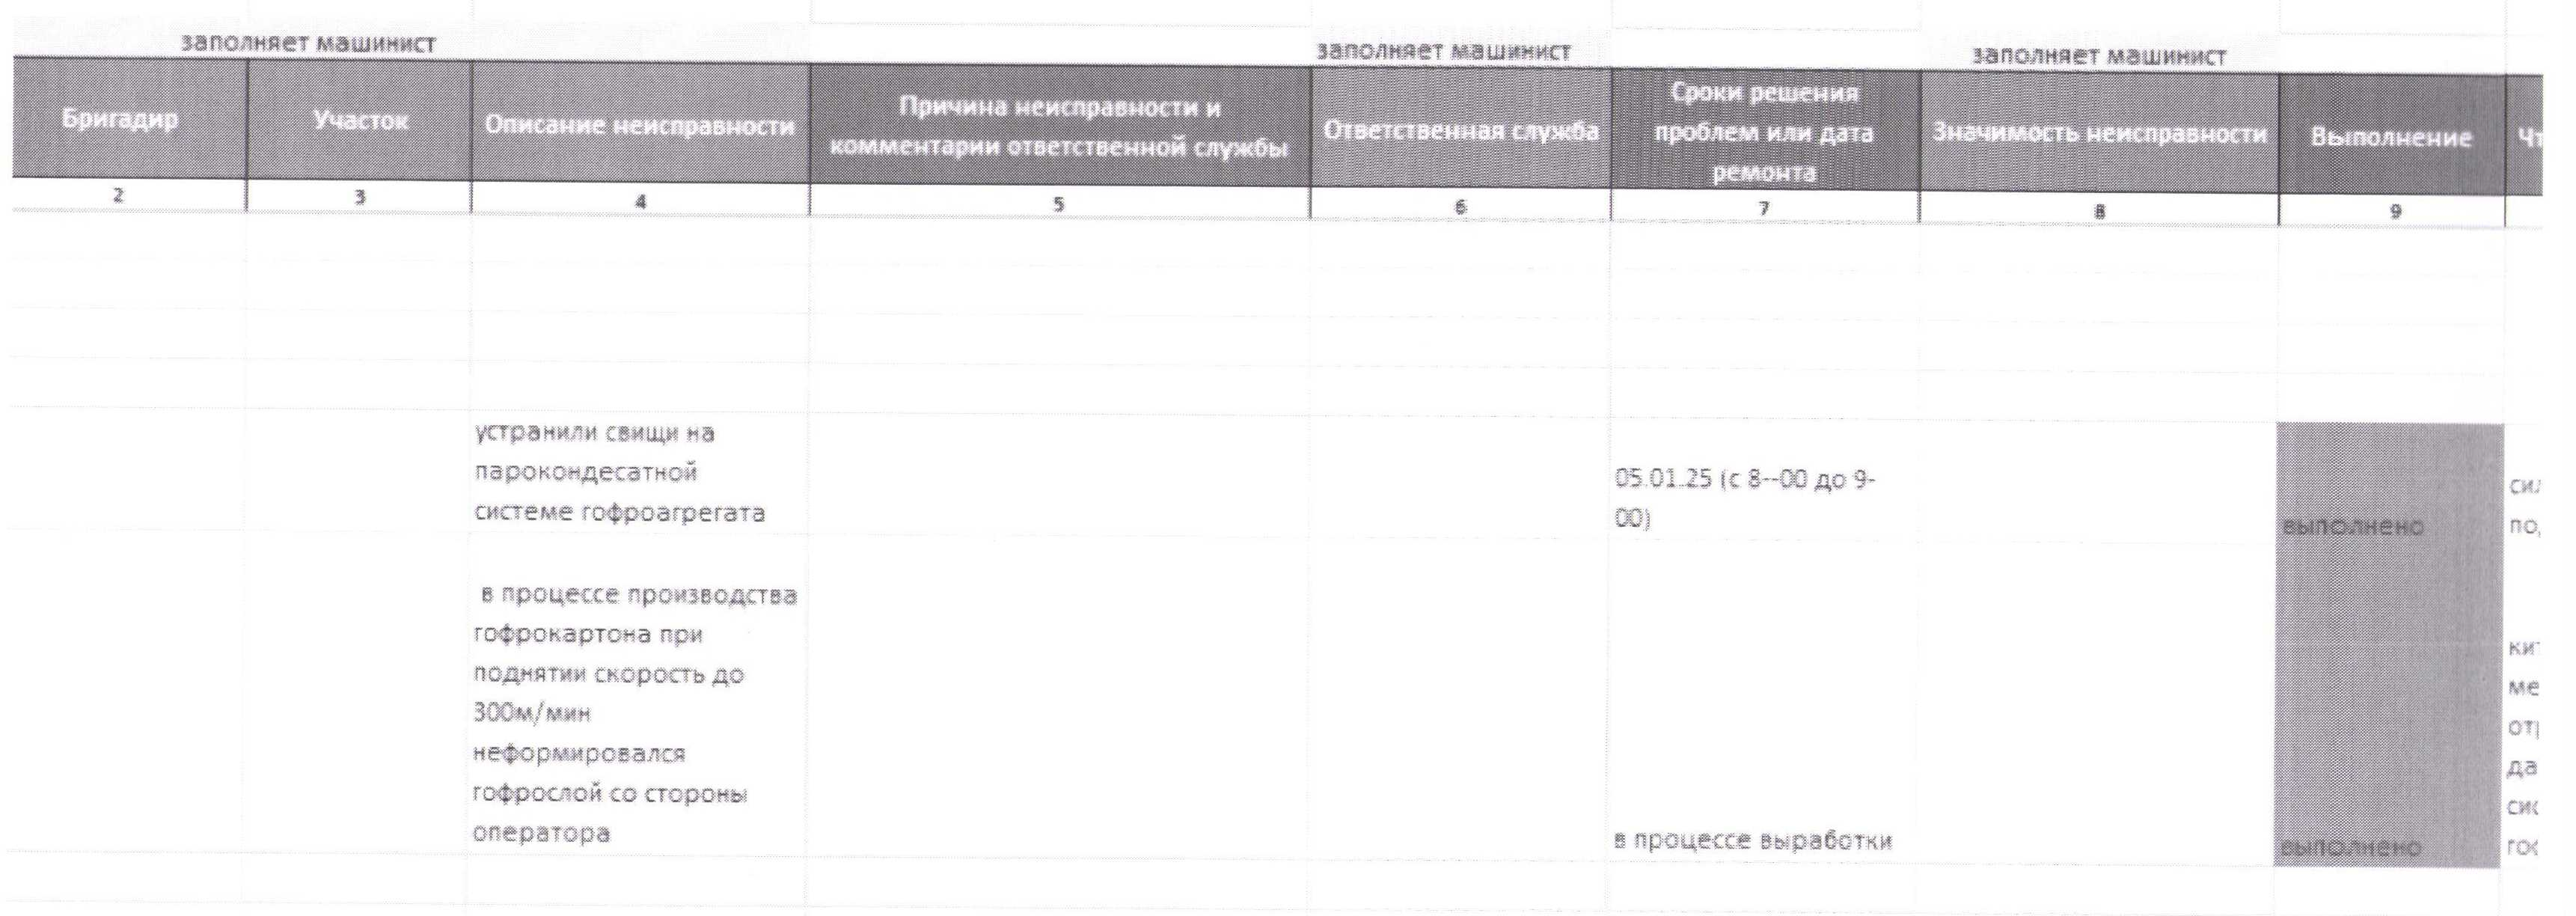
\includegraphics[height=0.94\textheight, width=\textwidth, angle=90, keepaspectratio]{Pics/f28.jpg}
\end{center}
\caption{Журнал простоев и неисправностей}
\label{pic:f28}
\end{figure}

\begin{figure}
\begin{center}
 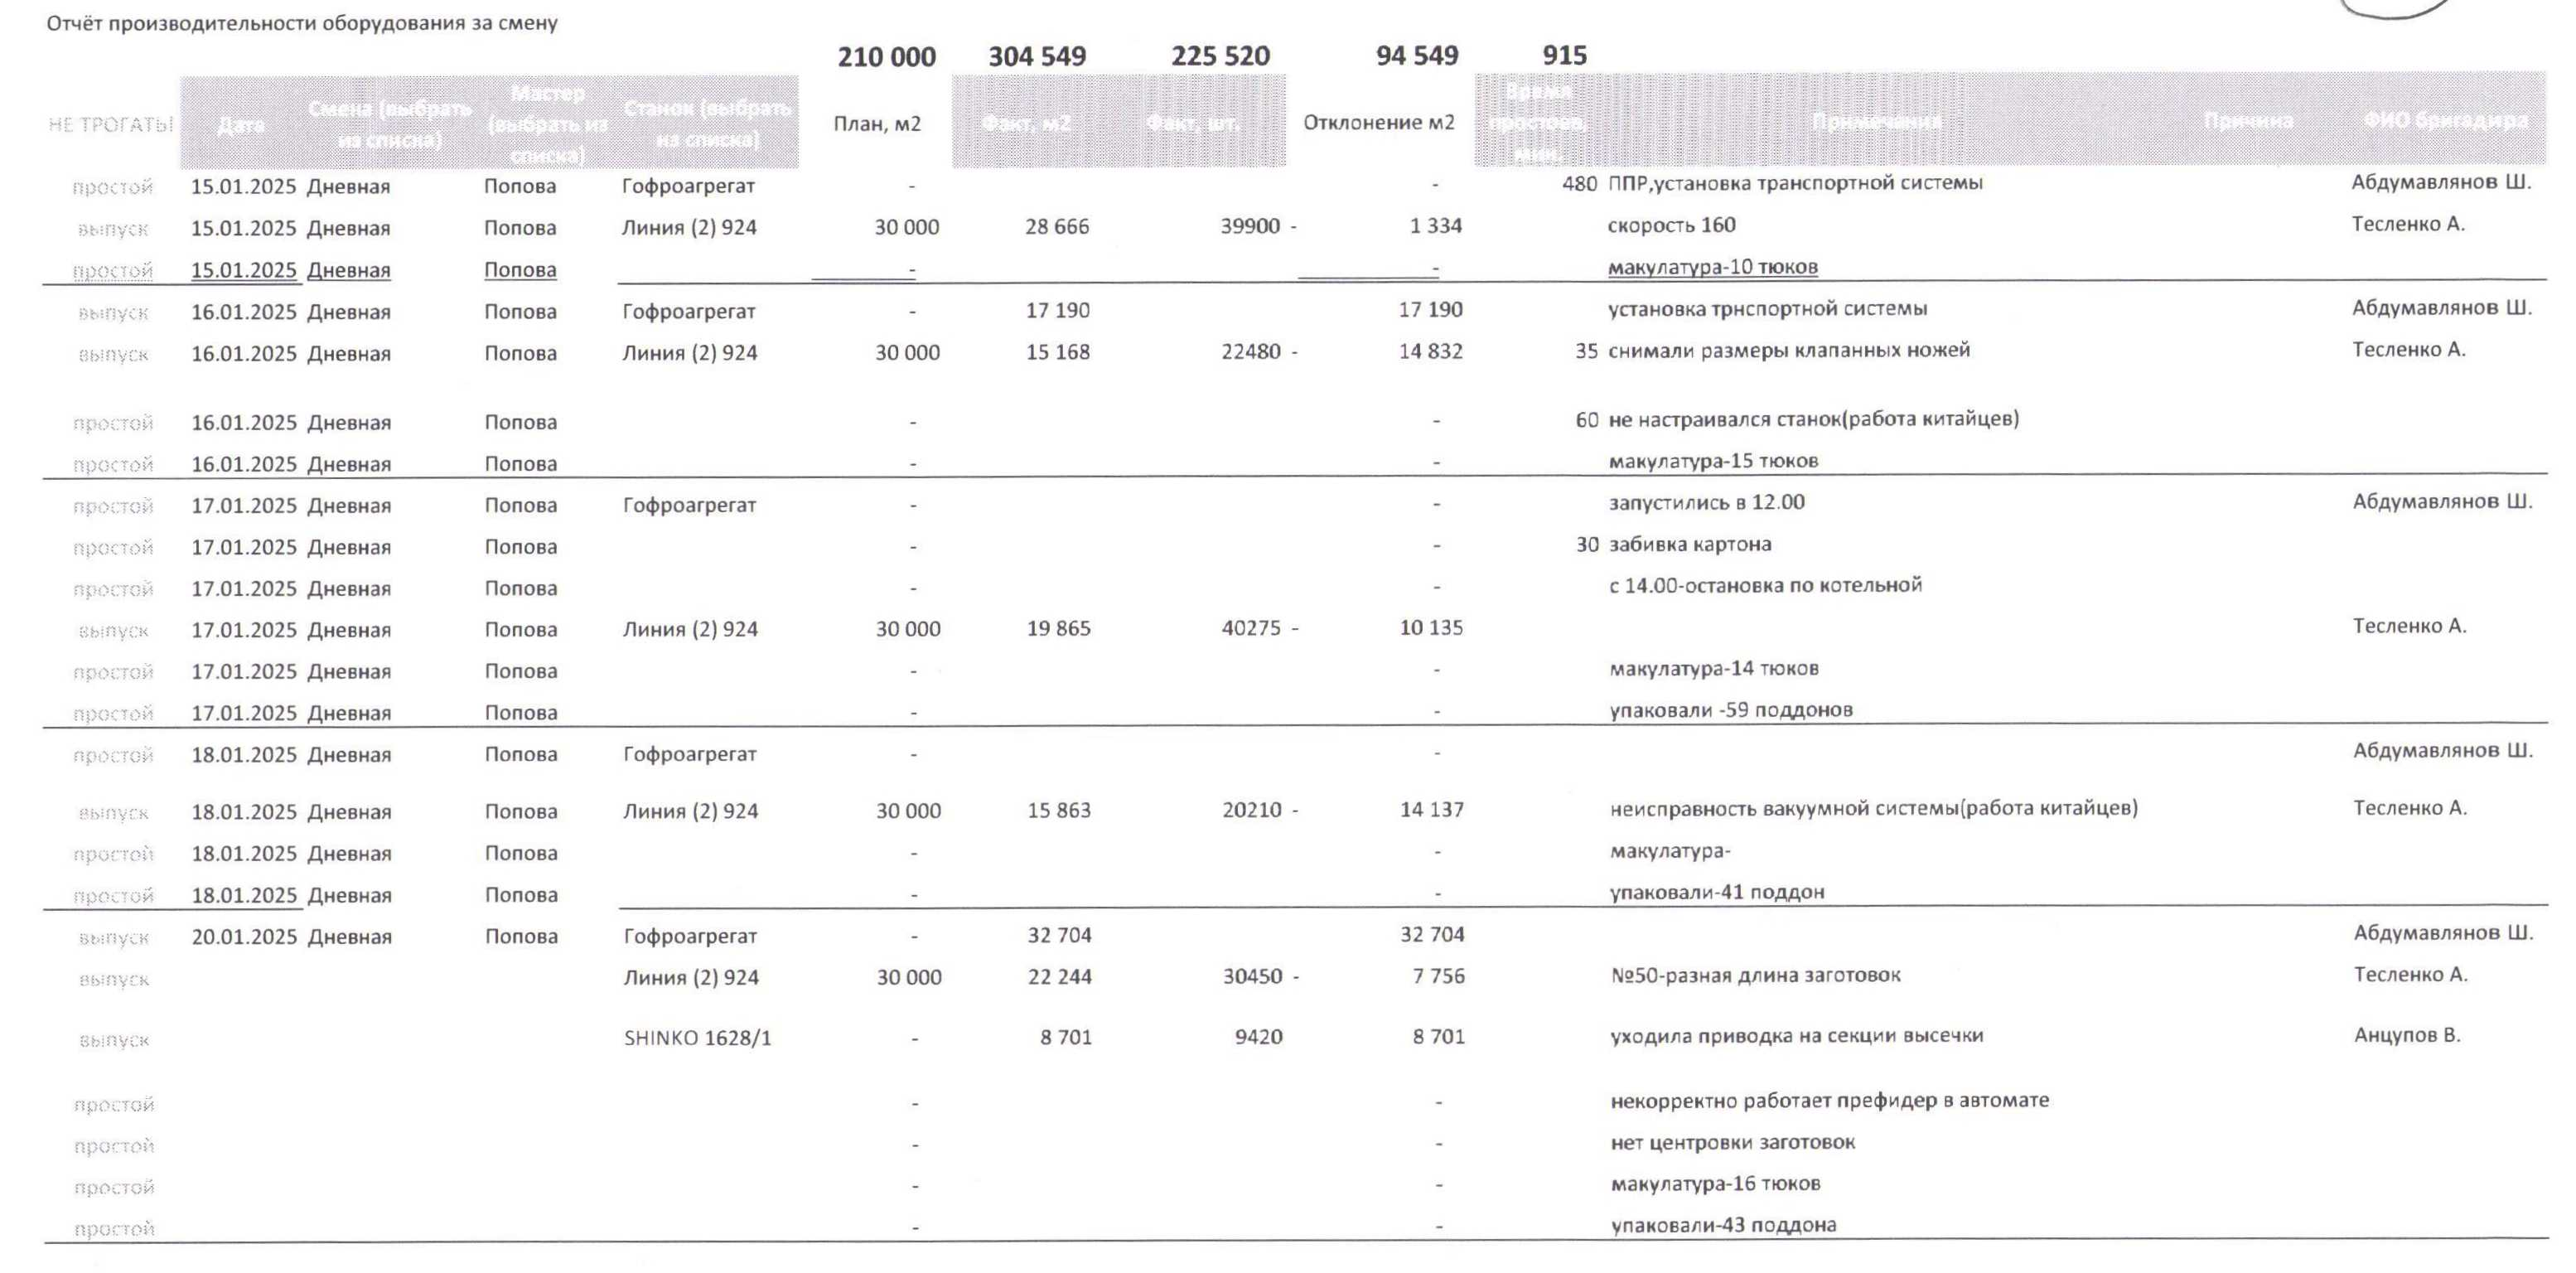
\includegraphics[width=\linewidth, height=0.94\textheight, keepaspectratio]{Pics/f25.jpg}
\end{center}
\caption{Отчет производства за смену ПЛ}
\label{pic:f25}
\end{figure}

\begin{figure}
\begin{center}
 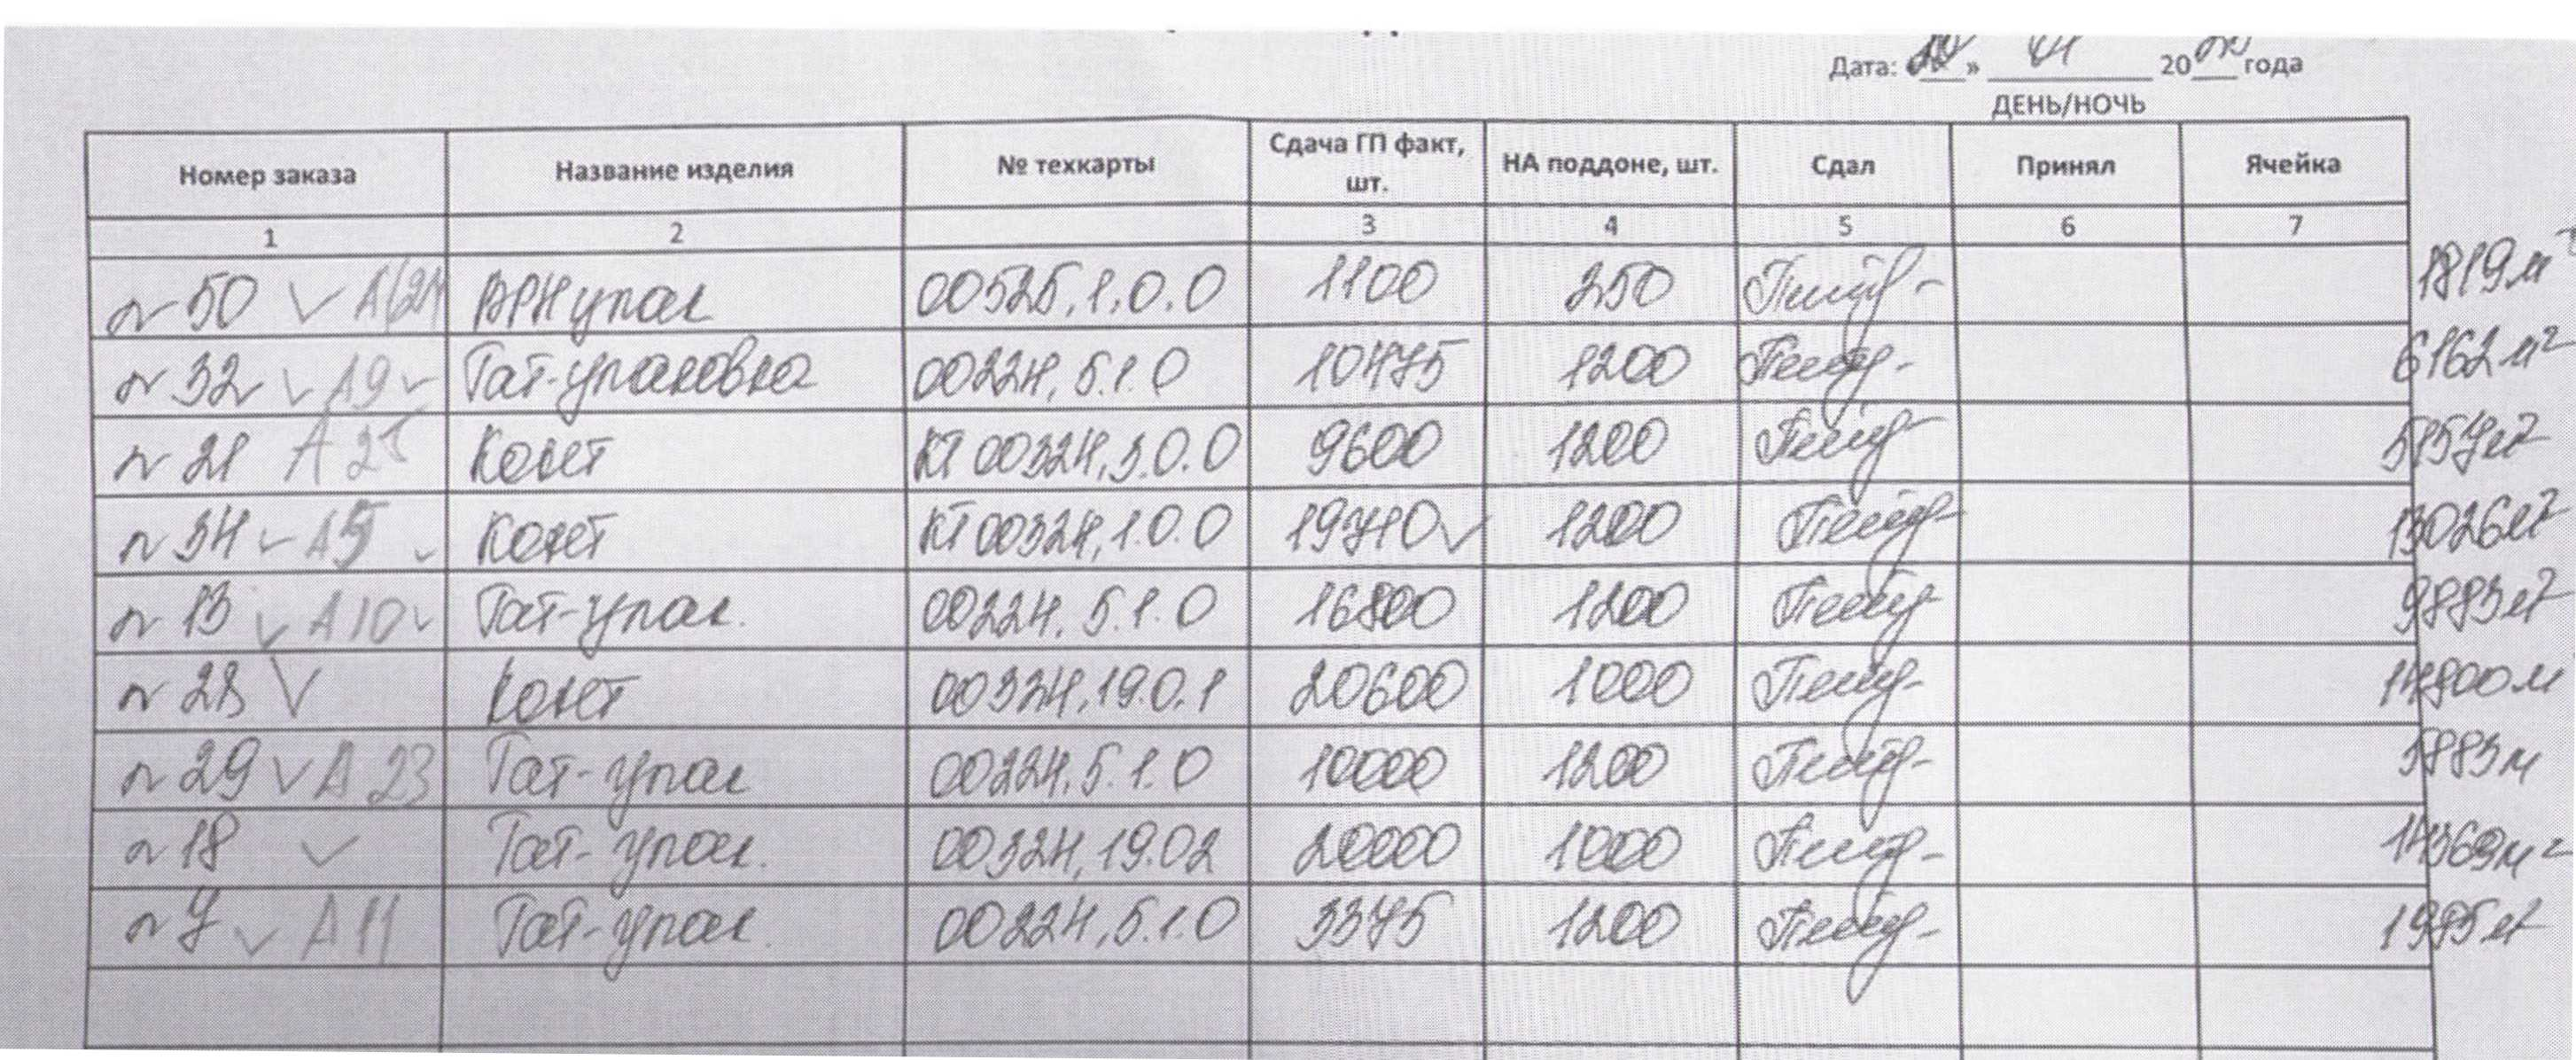
\includegraphics[width=\linewidth, height=0.94\textheight, keepaspectratio]{Pics/f6.jpg}
\end{center}
\caption{Ведомость передачи ГП на склад}
\label{pic:f6}
\end{figure}

\clearpage